\chapter{Il Protocollo}

In questo capitolo verrà trattato il protocollo proposto per l'implementazione
della Time-Lock Encryption sui DLT. Nella prima parte cercheremo di spiegare
l'idea che sta alla base, anche con l'ausilio di un esempio. Nella seconda parte
invece passeremo ad analizzare gli aspetti più formali, come le caratteristiche
dello Smart Contract che
serve implementare e i requisiti del DLT sui cui operare.

\section{L'idea}
\subsection{Versione base}
Immaginiamo che Carol abbia bisogno di Time-Lock Encryption su un certo messaggio $ x $.
Per farlo decide farsi aiutare da Alice. Quest'ultima
impegna a conservare il messaggio e ha renderlo pubblico solo dopo un
certo istante di tempo $ \tau $.
Immaginiamo inoltre che venga fissata una certa ricompensa da corrispondere ad Alice
per il suo servizio di conservazione di $ x $.

Alice vuole essere sicura di
ottenere la ricompensa se rispetta il suo impegno. Allo stesso tempo Carol
vuole avere la certezza che Alice possa riscattare il premio solo se si comporta
in maniera corretta.
Carol inoltre non vuole che soggetti terzi partecipino all'accordo, perché desidera
che sia $ x $ sia l'accordo stesso rimangano segreti.
Per farlo decidono di usare uno smart contract.

Nella fase iniziale Carol invia ad Alice il messaggio $ x $. Allo stesso tempo invia
allo smart contract una certa cifra in criptomoneta
che corrispone alla somma tra il premio \textit{prize} da corrispondere ad Alice e un
\textit{pawn} che le verrà ritornato al termine delle operazioni, un hash
crittografico del segreto $ x $ e l'istante di tempo $ \tau $.
\begin{figure}[H]
	\centering
	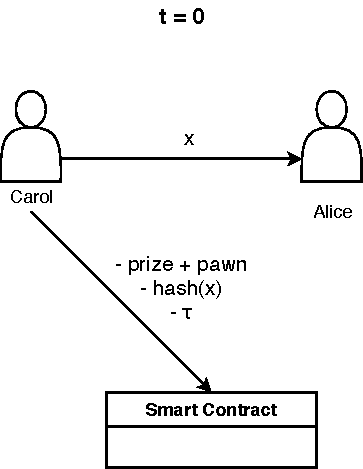
\includegraphics[width=0.3\linewidth]{images/chap_protocollo/step-0.pdf}
	\caption{Step 0}
\end{figure}


Alice si impegna quindi a conservare il segreto, e al tempo $ \tau $ lo rende noto.
Per farlo invia allo smart contract $ x $, ed in cambio ottiene il suo premio
\textit{price}.
Allo stesso tempo, Alice riottiene il \textit{pawn} che aveva versato in precedenza.
\footnote{Ad una prima analisi può sembrare che il \textit{pawn} sia inutile, 
ma in realtà è necessario per proteggersi da alcuni tipi di attacchi.
Le ragioni dettagliate verranno discusse nei capitoli successivi.}
\begin{figure}[H]
	\centering
	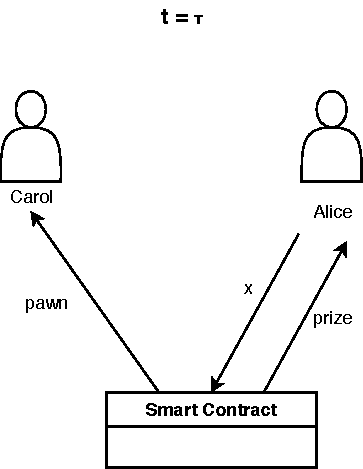
\includegraphics[width=0.3\linewidth]{images/chap_protocollo/step-ok.pdf}
	\caption{Step ok}
\end{figure}

Dopo che Alice ha inviato $ x $ allo smart contract, il messaggio diventa pubblico e 
chiunque può leggerlo.
\begin{figure}[H]
	\centering
	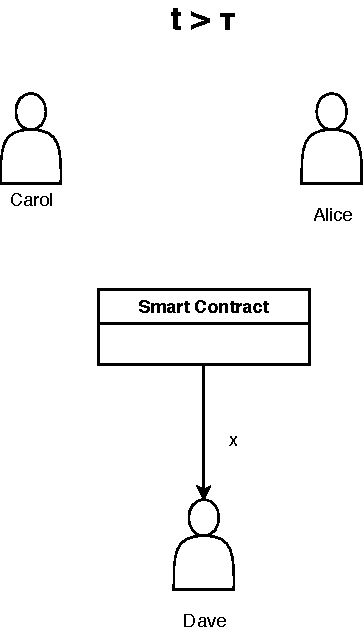
\includegraphics[width=0.3\linewidth]{images/chap_protocollo/step-leggi.pdf}
	\caption{Step leggi}
\end{figure}


Cosa succede se Alice prova a riscattare il premio prima dell'istante $ \tau $?
Semplicemente lo smart contract rifiuta la sua richiesta.
\begin{figure}[H]
	\centering
	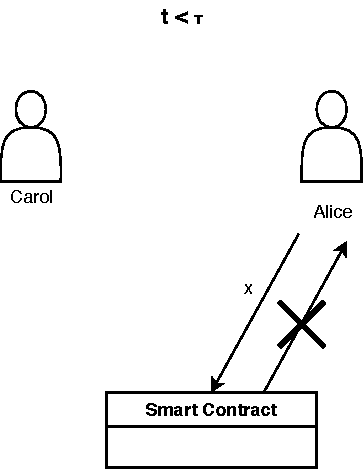
\includegraphics[width=0.3\linewidth]{images/chap_protocollo/step-anticipo.pdf}
	\caption{Step anticipo}
\end{figure}

E se Carol cedesse il segreto ad Eve prima del tempo $ \tau $?
In questo caso Eve usare $ x $ per ottenere un \textit{counterprize}. 
Ciò inoltre impedirebbe ad Alice di ottenere il suo premio. 
È evidente che l'interesse di Alice sia quello di mantenere $ x $ segreto
\begin{figure}[H]
	\begin{minipage}{0.5\textwidth}
        \centering
        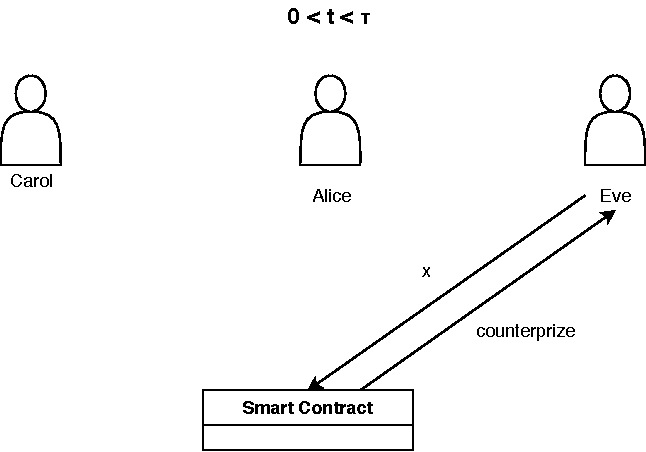
\includegraphics[width=.9\linewidth]{images/chap_protocollo/leak-1.pdf}
        \caption{Leak 1}
      \end{minipage}\hfill
      \begin{minipage}{0.5\textwidth}
        \centering
        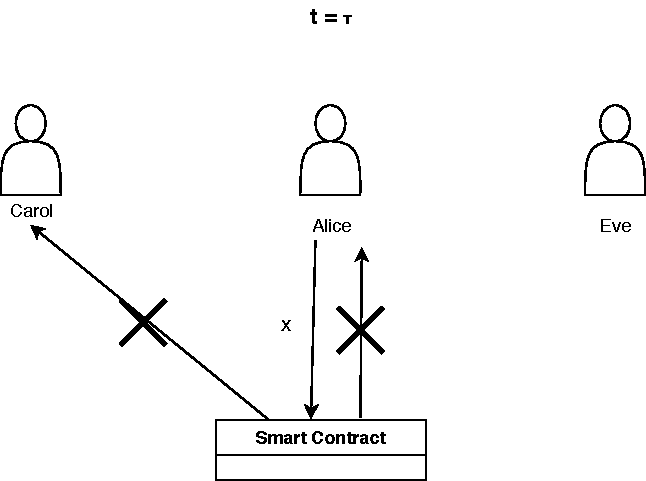
\includegraphics[width=.9\linewidth]{images/chap_protocollo/leak-2.pdf}
        \caption{Leak 2}
      \end{minipage}
\end{figure}


\subsection{Versione avanzata}
Facciamo notare che nello scenario di cui sopra Alice conosce sin 
dall'inizio il messaggio
$ x $, perché le è stato affidato nella prima fase del processo.
Ma se Carol volesse che il messaggio rimanga segreto anche ad Alice?
Per fare ciò Alice ha bisogno di (almeno) un altro collaboratore, Bob, e di un
algoritmo di \textbf{secret sharing}, \footnote{Un algoritmo di secret sharing
è un algoritmo che permette di
distribuire un certo segreto tra un gruppo di partecipanti, ad ognuno dei quali viene
assegnato uno \textit{share}. Il segreto può essere ricostruito solo unendo un certo
numero di share.}

